\documentclass[12pt,a4paper]{article}
\usepackage[T1]{fontenc}
\usepackage[swedish]{babel}
\usepackage[utf8]{inputenc}
\usepackage{lmodern}
\usepackage{listings}
\usepackage{hyperref}
\usepackage{graphicx}
\usepackage{color}

\begin{document}
	\title{\Huge Verksamhetsplan 2016}
	\author{Sportsektionen}
	\date{\today}

	\maketitle


	\begin{center}
		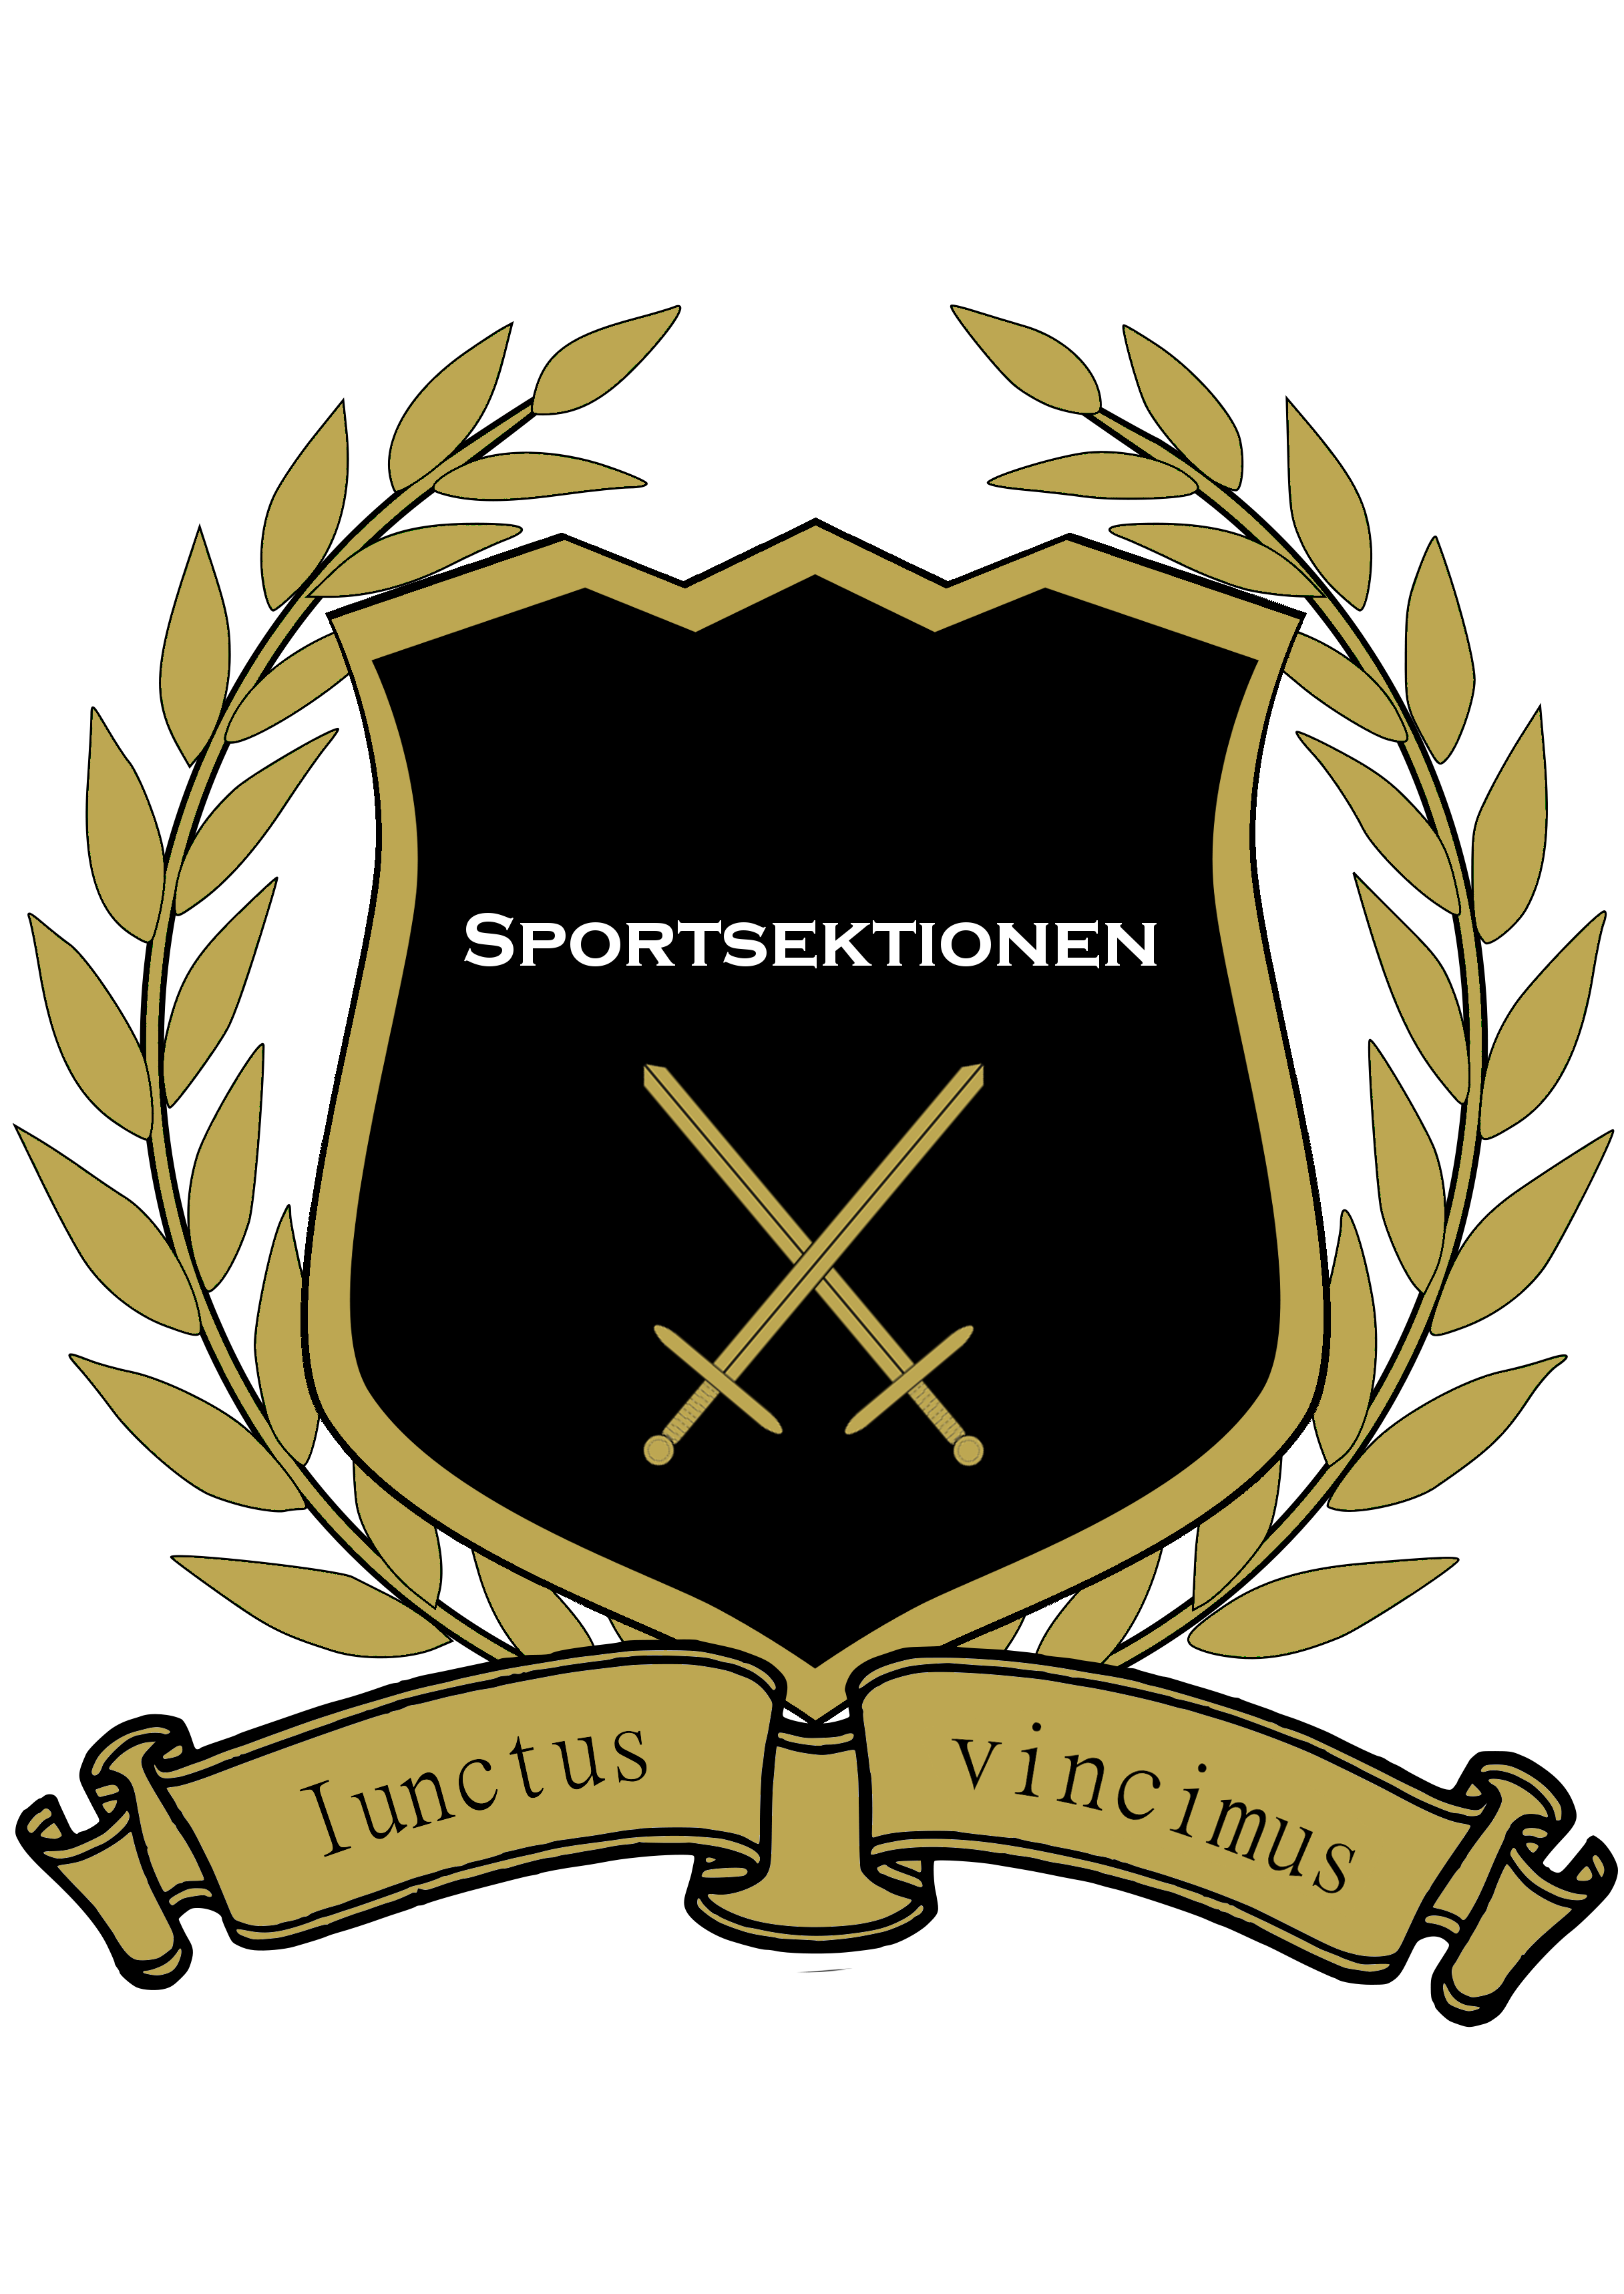
\includegraphics[scale=0.1]{../../Images/logo/logo}
	\end{center}


	\null
	\vfill

	\clearpage

	Under verksamhetsåret 2016 skall Sportsektionen verka för att främja studenthälsan för DISKs medlemmar genom återkommande evenemang, främst i form av sportaktiviteter.
	Sportsektionen skall verka för att ge DISKs medlemmar möjligheten att regelbundet spela badminton, innebandy, basket och fotboll i den utsträckning som DISKs medlemmar efterfrågar och som sektionen kan tillhandahålla.

	Sportsektionen ska tjäna sitt syfte så som det anges i sektionens stadgar och framför allt uppmuntra och verka för schysst spel och en kamratlig anda. Alla aktiviteter ska i allra största möjliga utsträckning vara tillgängliga och välkommnande för alla DISKs medlemmar oavsett kön. Sektionens aktiviteter ska också vara öppna för de som inte är medlemmar i DISK så länge det inte har en negativ inverkan på DIKSs ekonomi.

	Sportsektionen skall verka för ett ökat samarbete med andra studentkårer genom att delta i olika turneringar som anordnas och anordna egna turneringar. Sportsektionen skall också verka för fortsatt och ökat samarbete med övriga sektioner inom DISK, bland annat genom att medverka under Insparken. Sportsektionen skall verka för att planeringen av den traditionsenliga  resan till Åre Skiweek under vårterminen 2017 tar sin början. Sportsektionen skall även verka för att få sponsorer till sina aktiviteter.
\end{document}
